\section{Evaluation}
\label{sec_evaluation}
This section evaluates our automatic approach of checking the behavioral correctness of the metamodel and code co-evolution. 
First, we present the data set and the evaluation process. Then, we set the research questions we address and discuss the obtained results.


\begin{table*}[t]
\centering

		\caption{Details of the metamodels and their evolutions.}
		\label{CaseStudies_Evolution}
    \hspace*{-2em}
	\resizebox{14.5cm}{!} {
  \hspace*{-2em}
	\begin{tabular}{llll}
		\toprule
		 \begin{tabular}[c]{@{}l@{}}Evolved metamodels\end{tabular}                 & Versions & %\begin{tabular}[c]{@{}l@{}}Size ($N^{o}$ of\\ elements)\end{tabular} &
		\multicolumn{1}{c}{\begin{tabular}[c]{@{}c@{}}Atomic changes \\in the metamodel\end{tabular}} & \multicolumn{1}{c}{\begin{tabular}[c]{@{}c@{}}Complex changes \\in the metamodel\end{tabular}} \\ \midrule		

		%\multirow{6}{*}{\begin{tabular}[c]{@{}l@{}}OCL\end{tabular}} 
		\begin{tabular}[c]{@{}l@{}}Pivot.ecore \\ in project\\\emph{ocl.examples.pivot}\end{tabular}                        &  \begin{tabular}[c]{@{}l@{}}3.2.2 \\ to\\ 3.4.4\end{tabular}        &   %\begin{tabular}[c]{@{}l@{}}Original: 1473 \\Evolved: 1787\end{tabular}  &
		\begin{tabular}[c]{@{}l@{}} \emph{Deletes:} 2 classes, 16 properties, 6 super types \\ \emph{Renames:} 1 class, 5 properties \\ \emph{Property changes:} 4 types;  2 multiplicities \\ \emph{Adds:} 25 classes, 121 properties,  36 super types  \end{tabular}                                                         &    \begin{tabular}[c]{@{}l@{}} 1 pull property \\ 2 push properties  \end{tabular}                                                        \\ \midrule %cmidrule{2-5} %midrule	

\begin{tabular}[c]{@{}l@{}}Pivot.ecore \\ in project\\\emph{ocl.pivot}\end{tabular}                        &  \begin{tabular}[c]{@{}l@{}}6.1.0 \\to\\ 6.7.0 \end{tabular}        &    \begin{tabular}[c]{@{}l@{}} \emph{Deletes:} 0 classes, 4 properties, 4 super types \\ \emph{Renames:} 0 class, 1 properties \\ \emph{Property changes:} 49 types;  \\ \emph{Adds:} 5 classes, 47 properties,  7 super types  \end{tabular}    &   n/a \\ \midrule

    %\begin{tabular}[c]{@{}l@{}}Pivot.ecore in \\ project\\ocl.pivot\end{tabular}                        &  \begin{tabular}[c]{@{}l@{}}6.7.0 \\to\\ 6.18.0 \end{tabular}        &    \begin{tabular}[c]{@{}l@{}} \emph{Deletes:} 0 classes, 0 properties, \\ 0 super types \\ \emph{Renames:} 0 class, 1 properties \\ \emph{Property changes:} 5 types; \\  0 multiplicities \\ \emph{Adds:} 1 classes, 4 properties, \\ 1 super types  \end{tabular} & n/a   \\ 

    \begin{tabular}[c]{@{}l@{}}ExtendedTypes.ecore \\in project\\\emph{papyrus.infra.extendedtypes}\end{tabular}            & \begin{tabular}[c]{@{}l@{}}0.9.0 to\\ 1.1.0\end{tabular}         & %\begin{tabular}[c]{@{}l@{}}Original: 40 \\Evolved: 57\end{tabular}     &   
		\begin{tabular}[c]{@{}l@{}}Deletes: 10 properties, 2 super types \\ Renames: 3 classes, 2 properties \\ Adds: 8 classes, 9 properties, 8 super types  \end{tabular}                                                      &    \begin{tabular}[c]{@{}l@{}} 2 pull property \\ 1 push property \\ 1 extract super class \end{tabular} \\ \midrule

  \begin{tabular}[c]{@{}l@{}}Benchmark.ecore \\ in project \\ \emph{modisco.infra.discovery.benchmark}\end{tabular}                & \begin{tabular}[c]{@{}l@{}}0.9.0 to\\ 0.13.0\end{tabular}         &   %\begin{tabular}[c]{@{}l@{}}Original: 95 \\Evolved: 106\end{tabular}    &  
		\begin{tabular}[c]{@{}l@{}} Deletes: 6 classes, 19 properties, 5 super types \\ Renames: 5 properties  \\ Adds: 7 classes, 24 properties, 4 super types  \end{tabular}                                                        &     \begin{tabular}[c]{@{}l@{}} 4 moves property \\ 6 pull property \\ 1 extract class \\ 1 extract super class \end{tabular}    
   \\ \midrule
   \midrule

  \begin{tabular}[c]{@{}l@{}}Ecore.ecore \\ in project \\ \emph{org.eclipse.emf}\end{tabular}                & \begin{tabular}[c]{@{}l@{}}2.37.0 to\\ 2.37.0'\end{tabular}         &   %\begin{tabular}[c]{@{}l@{}}Original: 95 \\Evolved: 106\end{tabular}    &  
		\begin{tabular}[c]{@{}l@{}} Deletes: 1 class, 2 properties \\ Renames: 2 properties  \\   \end{tabular}                                                        &     \begin{tabular}[c]{@{}l@{}} 1 move property \\ 1 pull property  \end{tabular}    
  \\ 
  
  \bottomrule                                         
	\end{tabular}
}
%\vspace{-1em}
\end{table*}


\subsection{Data Set}
 
This section presents the used data set in our evaluation to be found in the attached supplementary material\footnote{\url{https://figshare.com/s/b6251b9e47fa82983ce5}}. 



We evaluate our approach on four case studies of language implementations in Eclipse, namely OCL \cite{MDTOCL}, Modisco \cite{MDTModisco}, Papyrus \cite{MDTPapyrus}, and EMF \cite{EclipseEMF} project. 
%
OCL is a standard language defined by the Object Management Group (OMG) to specify First-order logic constraints. Modisco is an academic initiative to support development of model-driven tools, reverse engineering, verification, and transformation of existing software systems. 
Papyrus is an industrial project led by CEA\footnote{\url{http://www-list.cea.fr/en/}} to support model-based simulation, formal testing, safety analysis, etc. 
\red{The EMF project is a modeling framework and code generation facility for building tools and other applications based on a structured data model \cite{steinberg2008emf}.}  
Thus, the four case studies cover standard, academic, and industrial languages that have evolved several times for more than 10 years of continuous development period. 

Moreover, we aimed at selecting meaningful evolutions that do not consist in only deleting metamodel elements, but rather include complex evolution changes. We also aimed to select long and short evolution intervals in the selected releases versions to stress test our approach in different scenarios. 
\red{This is the case for the OCL, Modisco, and Papyrus case studies. However, they do not have manually written tests. Thus, we added the EMF case study that have manually written tests, but its metamodel is stable with no evolutions. Therefore, we had to simulate a set of metamodel evolution changes similar to those real-world changes observed in our three first case studies and we co-evolved their impacts with our previous work  \cite{Khelladi2020}.} 


Table \ref{CaseStudies_Evolution} gives details about the selected case studies, in particular about their metamodels and the changes applied during evolution. 
%\red{Also about the code and tests details in each project.}
The total of applied metamodel changes was \red{452} atomic changes and \red{21} complex changes in the five metamodels.
%
Table~\ref{CaseStudies_CoEvolution} gives details on the size of the projects in terms of code and tests of the original and evolved versions. 
We collected a total of~18 projects to evaluate our approach on.  



\subsection{Evaluation Process}

\red{We evaluate our approach by: 1) investigating its usefulness compared to the manual tracing of the impacted tests with user study, 2) measuring its ability to automatically trace the impacted tests due to impacting metamodel changes both in the original and evolved version of the project, 3) assessing its ability to give an indication about the correctness of the code and metamodel co-evolution, and finally 4) measuring the gains of its usage in terms of reduction of tests and their execution time.} Note that as the metamodel changes are taken as input of our automatic test tracing, we studied the original and evolved versions to confirm the metamodel changes. Therefore, we do not take an incorrect input of metamodel changes that would mislead our traced tests, which would mislead the behavioral checking of the code co-evolution. 


\red{Regarding the tests, only the EMF case study had manually written tests. Thus, we had to generate tests for OCL, Modisco, and Papyrus case studies. We used 
a state-of-the-art tool, namely EvoSuite~\cite{fraser2011evosuite}. 
EvoSuite is a search-based tool for Unit Tests generation. It uses a heuristic algorithm, particularly, genetic algorithm
% ( explain different elements of it ?)
in the Test Suit generation. In their used approach Fraser et al.~\cite{fraser2011evosuite} aimed to maximize the coverage metric and mutation score which guarantees good-quality tests. 
EvoSuite is largely used and it was evaluated not only in literature but also in the industrial context. Firhard et al.~\cite{10.1007/978-3-031-21251-2_2} compared it with DSpot, a state-of-the-art tool for test amplification, their results show that EvoSuite achieves a statistically better mutation score. Herculano et al. found that EvoSuite's generated tests can successfully help to identify faults during maintenance tasks~\cite{9954000}. In industry, Rozière et al. use automated tests generated with EvoSuite to filter invalid code translations in the context of their work done for Meta \cite{roziere2021leveraging}. 
Gruber et al.~\cite{gruber2023automatic} further showed the quality and robustness of the generated tests. It showed that while flakiness is at least as common in generated tests as in developer-written tests, EvoSuite is effective in alleviating this issue giving~71.7\% fewer flaky tests. Thus, EvoSuite is appropriate in our work to generate robust tests in the original code and in the co-evolved code to compare their results, i.e., check behavioral correctness.} 
We simply let EvoSuite run to generate Junit test classes for the selected projects with the following parameters: \emph{-DmemoryInMB=2000 -Dcores=4 -DtimeInMinutesPerClass=10 evosuite:generate evosuite:export}. It uses up to 2GO of RAM, 4 CPU cores, and 10 minutes per test class. 
Generating tests is a best practice, in particular w.r.t. its efficiency in test generation and at a large scale for all public methods \cite{DANGLOT2019110398,https://doi.org/10.1002/stvr.1601}. 
EvoSuite generates tests for all public methods, whereas developers tend to manually write a few tests for only some targeted methods. Thus, relying only on manually written tests increases the risk of not assessing the behavioral correctness of many cases of code co-evolutions that are not covered by test cases. Generating tests alleviates this risk. 
\red{Indeed, this is observed when computing the coverage metric for each of our considered projects. Table \ref{table:coverage} shows that the highest coverage (69\% to 95\%) is obtained on projects with automatically generated tests and the lowest coverage (17\% to 33\%) were on the two projects with manually written tests.}  






\begin{table*}[t]
\centering
		\caption{Details of the projects and their tests.}
		\label{CaseStudies_CoEvolution}
  \hspace*{-2em}
	\resizebox{14.5cm}{!} {
	\begin{tabular}{lcccccc}
		\toprule
		\begin{tabular}[c]{@{}l@{}}Projects co-evolved in response to the evolved \\ metamodels \end{tabular} 	& \begin{tabular}[c]{@{}c@{}}$N^{o}$ of \\ packages\end{tabular} & \begin{tabular}[c]{@{}c@{}}$N^{o}$ of \\ classes\end{tabular} & %\begin{tabular}[c]{@{}c@{}}N° of \\ methods\end{tabular} & 
  \begin{tabular}[c]{@{}c@{}}$N^{o}$ of test\\ packages\end{tabular} & \begin{tabular}[c]{@{}c@{}}$N^{o}$ of test\\ classes\end{tabular} &
		\begin{tabular}[c]{@{}c@{}}$N^{o}$ of \\ LOC\end{tabular} & \begin{tabular}[c]{@{}c@{}}$N^{o}$ of \\ tests\end{tabular} %& \begin{tabular}[c]{@{}c@{}}$N^{o}$ of total \\ direct errors \end{tabular}& \begin{tabular}[c]{@{}c@{}}$N^{o}$ of total \\ indirect errors \end{tabular}
  \\ \midrule		

$[P1_{V1}]$ ocl.examples.pivot & 22 & 439 &22  & 290 & 74002 & 7322 \\ \midrule

$[P1_{V2}]$ ocl.examples.pivot & 22 & 480 & 22 &220 &  89449& 4990 \\ \midrule

$[P2_{V1}]$ ocl.examples.base & 12 & 181 & 12 &119 &17617 & 2320 \\ \midrule

$[P2_{V2}]$ ocl.examples.base & 12 & 181 & 12 & 118&17596 & 2133 \\ \midrule


$[P3_{V1}]$ ocl.pivot & 60 & 1006 & 55 &598 & 142236& 8795 \\ \midrule

$[P3_{V2}]$ ocl.pivot & 63 & 1090 & 58 & 683&153613 & 6396 \\ \midrule

%$[P3_{V3}]$ ocl.pivot & 66 & 1143 & 61 & 738&164845 & 6356 \\ \midrule

$[P4_{V1}]$ papyrus.infra.extendedtypes & 7 & 37 &7  & 19 & 2057 & 135 \\ \midrule

$[P4_{V2}]$ papyrus.infra.extendedtypes & 7 & 51 & 7 &26 &  2570 & 248 \\\midrule
$[P5_{V1}]$ papyrus.infra.extendedtypes.emf & 5 & 25 &4  & 14 & 1145 & 104 \\ \midrule

$[P5_{V2}]$ papyrus.infra.extendedtypes.emf & 5 & 25 & 4 &14 &  1145& 104 \\ \midrule
$[P6_{V1}]$ papyrus.uml.tools.extendedtypes & 5 & 15 &3  & 9 & 726 & 75 \\ \midrule

$[P6_{V2}]$ papyrus.uml.tools.extendedtypes & 5 & 15 & 3 &9 &  725& 75 \\ \midrule

$[P7_{V1}]$ org.eclipse.modisco.infra.discovery.benchmark & 3 &  28& 3 &15 & 2333 &524  \\ \midrule

$[P7_{V2}]$ org.eclipse.modisco.infra.discovery.benchmark &3  & 30 &3  & 15&  2588& 619 \\%\midrule


		% \begin{tabular}[c]{@{}l@{}}$[P1]$ ocl.examples.pivot\\ $[P2]$ ocl.pivot\end{tabular}      &   \begin{tabular}[c]{@{}l@{}}22\\// \end{tabular}     & \begin{tabular}[c]{@{}l@{}}439\\?? \end{tabular}                 &                                          %  \begin{tabular}[c]{@{}l@{}}5445\\1984 \end{tabular}              & 
		%\begin{tabular}[c]{@{}l@{}}74002\\// \end{tabular} & \begin{tabular}[c]{@{}l@{}} ??\\?? \end{tabular} %& \begin{tabular}[c]{@{}l@{}} 489\\27 \end{tabular} & \begin{tabular}[c]{@{}l@{}} 37\\2 \end{tabular} 
  %\\ \midrule	
  
		% \begin{tabular}[c]{@{}l@{}}$[P1]$ ocl.examples.pivot\\ $[P2]$ ocl.pivot\end{tabular}      &   \begin{tabular}[c]{@{}l@{}}22\\// \end{tabular}     & \begin{tabular}[c]{@{}l@{}}439\\?? \end{tabular}                 &                                          %  \begin{tabular}[c]{@{}l@{}}5445\\1984 \end{tabular}              & 
		%\begin{tabular}[c]{@{}l@{}}74002\\// \end{tabular} & \begin{tabular}[c]{@{}l@{}} ??\\?? \end{tabular} %& \begin{tabular}[c]{@{}l@{}} 489\\27 \end{tabular} & \begin{tabular}[c]{@{}l@{}} 37\\2 \end{tabular} 
  %\\ %\midrule	
\midrule		
\midrule
$[P_{ecore\_V1}]$ org.eclipse.emf.ecore & 13 & 168& /& / & 142586 & 0 \\
\midrule
$[P_{ecore\_V2}]$ org.eclipse.emf.ecore & 13 & 166 & /  & / & 141434 & 0 \\ 

\midrule
		
		
$[P8_{V1}]$ org.eclipse.emf.test.core & / & / &19 & 141 & 40858 & 322 \\
\midrule
$[P8_{V2}]$ org.eclipse.emf.test.core & / & / &19  & 141 & 40544 & 322 \\ 

\midrule
		
$[P9_{V1}]$ org.eclipse.emf.test.xml & / & / & 6& 27 & 12088 & 64 \\
\midrule
$[P9_{V2}]$ org.eclipse.emf.test.xml & /& / &6  & 27 & 12088 & 64 \\ 


   \bottomrule		
	\end{tabular}
}

\end{table*}

\begin{table*}[t]
%\begin{wraptable*}{r}{5.5cm}
\centering
\caption{Coverage metric of each evaluation project.} 
\label{table:coverage}
%
%\small
%\hspace*{-2em}
\resizebox{11cm}{!}{
\begin{tabular}{
@{\hskip3pt}c@{\hskip3pt}|c@{\hskip3pt}|c@{\hskip3pt}|c@{\hskip3pt}|c@{\hskip3pt}|c@{\hskip3pt}|c@{\hskip3pt}|c@{\hskip3pt}|| c@{\hskip3pt} |c@{\hskip3pt} }
\toprule 
Projects
& \begin{tabular}[c]{@{}l@{}}$[P1]$ \end{tabular}
& \begin{tabular}[c]{@{}l@{}}$[P2]$ \end{tabular} &\begin{tabular}[c]{@{}l@{}} $[P3]$  \end{tabular}
&\begin{tabular}[c]{@{}l@{}} $[P4]$\end{tabular}
&\begin{tabular}[c]{@{}l@{}} $[P5]$\end{tabular}
& \begin{tabular}[c]{@{}l@{}}$[P6]$ \end{tabular} 
& \begin{tabular}[c]{@{}l@{}}$[P7]$ \end{tabular}
&\begin{tabular}[c]{@{}l@{}}$[P8]$ \end{tabular}
&\begin{tabular}[c]{@{}l@{}}$[P9]$ \end{tabular}\\ \midrule%{2-10}


\begin{tabular}[c]{@{}l@{}}Coverage V1 \end{tabular} &  66.9\%  &  86.1\%    &   80.1\%  &  95.6\%  &   95.1\%    &   89.5\%   &   91.3\% &  18\%  &  33.4\%   \\ 
 \midrule%{2-10}


\begin{tabular}[c]{@{}l@{}}Coverage V2 \end{tabular} &  66.2\%  &  85.4\%    &   74.1\%  &  95.2\%  &   95.2\%    &   89.2\%   &   87.5\% &   17.2\% &  33\%    \\ 


\bottomrule
\end{tabular}
}
%\end{wraptable*} 
%\vspace{-1em}
\end{table*}

\subsection{Research Questions}
This section sets the research questions (RQs) to assess our work. The research questions are as follows:


\textbf{\emph{RQ0.}} \red{\emph{To what extent can developers manually trace the tests impacted by the evolution of the metamodel?}
This aims to asses if developers can manually trace the tests that are impacted by the changes of the metamodel.
This also aims further to assess our approach’s usefulness through main observations.} 

\textbf{\emph{RQ1.}} \red{\emph{To what extent does our automatic approach trace the impact of the metamodel evolution to the tests?} This aims to assess on real-world case studies the ability and applicability of our automatic approach to trace the metamodel changes with code elements till their tests.}  %This assesses the overall applicability of our co-evolution approach.  
    
\textbf{\emph{RQ2.}} \emph{What is the observed behavioral correctness level of the code co-evolution?} This aims to assess through running the selected tests the effect of the code co-evolution, whether it keeps the tests' results stable, or instead degrade or improve them. %\todo{here if you mapp them, we can look at the different cases}


\textbf{\emph{RQ3.}} \emph{What are the observed gains (w.r.t. test case reduction and execution time) obtained from our approach of tracing impacted tests by metamodel evolution ?} This aims to highlight the benefit of our approach compared to when not using it and relying on the whole test suite as a baseline. 


\subsection{Results}
We now discuss the results w.r.t. our research questions.

\red{


\subsubsection{RQ0}
The first goal of our evaluation is to gain evidence on the difficulty or not of the manual task of tracing impacted tests. Thus, we designed and ran a user study experiment. 

\paragraph{RQ0 Set Up} We first describe our user study experiment.

\textbf{Subjects selection.}
The experiment was conducted with 8 participants (2 females and 6 males), including PhD students and research engineers in IRISA Laboratory, at the University of Rennes. The participants have a varying level of experience in programming (from~3 to~12 years with an average of~7 years), and a varying level in model-driven engineering (MDE) (from 0 to 7 years with an average of~2 years and 6 months).

\textbf{Experiment Task.} 
The experiment aims to evaluate the ability of participants to trace manually and analyze the affected unit tests before and after the metamodel evolution.
We prepared two Eclipse workspaces. The first one contains the original version of the project \texttt{org.eclipse.emf.test.core}, and the second workspace contains the evolved version of the same project. 
The number of tests is 322 in both versions. The number of tests that must be traced is respectively 173 and 17 in the original and evolved versions. 
We then give in the guideline of the experiment the list of the changes that details the evolution of the metamodel (see last row of Table~\ref{CaseStudies_Evolution}) with a description of the metamodel and project. We also explain what type of code elements are generated from each metamodel element.
Each participant had then to identify impacted unit tests in the original and evolved version of the project \texttt{org.eclipse.emf.test.core}. This procedure not only highlights the direct impacts of the metamodel changes but also requires the consideration of indirect impacts. Additionally, the study explores the usefulness and potential adoption of our approach as an automatic support tool for tracing the impacted tests. 
After the end of this task, we presented our automatic tracing approach to the participant then we ran a post-questionnaire.

\textbf{Variables.} Our user study aimed to measure to what extent can developers trace impacted tests. The independent variable we controlled was the impacting metamodel changes. We covered seven different types of changes with both atomic and complex changes. 
We then observed the dependent variable of the traced tests by the participants. 

\paragraph{RQ0 Results}
When we analyzed the answers of each participant, we found that they were able to trace only a few tests. In the original version of the project, the total number the manually traced tests varied between~1 and~18, with an average of~6 tests out of the~173 impacted tests.   
In the evolved version of the project, the total number the manually traced tests varied between~2 and~32, with an average of~11 tests out of the~17 impacted tests.   
While we first observe that none of the participants traced all tests, they also did not correctly trace the tests. 

Indeed, the number of correctly manually traced tests varies between~1 to~18 in the original version of the project, with an average of~5 traced tests. In the evolved version, the number of correctly manually traced tests varies between~0 to~10 tests with an average of~4 tests. 
We had five participants out of eight who wrongly traced eight tests in the original version of the projects, varying between one or two tests for each of them. In the evolved version of the project, all participants have wrongly traced between one to 26 tests that are not impacted by the evolution of the metamodel. 
We investigated the cause of this incorrect tracing. We found that one reason was the tracing  of tests that contain a commented impacted code. 
Another reason was traced the wrong overload method \texttt{getEEnumLiteral(EInt)} of the actually evolved method \texttt{getEEnumLiteral(EString)}. Another reason was to simply include sibling tests in the class of a trace test. 
%Considering that the method \texttt{getEEnumLiteral} with \textit{EString} as type parameter, located in  the class \texttt{EEnum} to \texttt{getEEnumLiteralV2}, and that this renamed method is overloaded with \textit{EInt} as parameter type.
%Two other participants traced in the original version of the project, and by confusion, tests that uses \texttt{getEEnumLiteral} with \textit{EInt} as parameter type.

In addition, we found that five participants considered both the direct and indirect impact of the metamodel evolutions on the tests, while the 3 remaining participants considered only the directly impacted tests. 
%
The results of the user study show the difficulty of manually tracing the tests with the evolved metamodel. Not only the participants could not trace all tests, but they even wrongly traced non-necessary tests. 

Regarding the answers of the participants about usefulness\footnote{Between 'Useless – Little useful – Somewhat useful – Very useful – Extremely useful'.} of our approach as an automatic support tool for tracing the impacted tests. One participant graded our approach as 'Somewhat useful', five out of eight graded it as 'Very useful', and two graded it as 'Extremely useful'. The last question was about their potential adoption\footnote{Between 'Very unlikely - Unlikely - Somewhat likely - Likely - Very likely'.}%\footnote{Between '1 - 2 - 3 - 4 - 5' (1 for least potential adoption, and 5 for highest potential adoption).} 2 of 3, 3 of 4, 3 of 5
of our approach as an automatic support tool for tracing the impacted tests. Two participants out of eight answered 'Somewhat likely', three participants answered 'Likely', and the three remaining participants answered 'Very likely'. The finding of this experiment emphasizes the adoption likelihood and usefulness of our approach (discussed in RQ4).

\begin{tcolorbox}[boxsep=-2pt]
\textbf{$\boldsymbol{RQ_0}$ insights:}
 From our user study experiment, we observe that tracing manually the tests impacted by the evolution of the metamodel is a hard and error-prone task. The post-questionnaire results after a demonstration of our automatic approach suggest its high usefulness and adoption likelihood.
\end{tcolorbox}

}

\subsubsection{RQ1}

Following the evaluation protocol, we executed our approach on our case studies in Table \ref{CaseStudies_CoEvolution}. Figure \ref{fig:tracedTests} depicts the number of traced tests due to the impacting metamodel changes in Table \ref{CaseStudies_Evolution}. We first observe that we can trace tests successfully. We traced a total of \red{1608 out of 34612 tests due to 473 metamodel changes, distributed in 1106 and 502 tests} in the original and evolved versions. Thus, we can isolate for the developers the tests that must be executed and looked at to check the behavioral correctness of the co-evolution. 

We also observe that the more the number of evolution changes between the original and evolved versions of the metamodel increases,  the more the number of tests we trace increases as well. In particular, when a lot of tests are available for analysis. This is true for the OCL Pivot project $[P1]$ and Modisco project $[P1]$. \red{We also observe no overall difference between projects with automatically generated tests and projects with manually tests. We traced similar ratios of tests.} 

Moreover, as several deletions of classes and properties occurred in the evolution changes, several tests are not generated in the evolved version, which explains why we trace more tests in the original version than in the evolved version. This is observed in most of the projects except the $[P4]$, where $[P4_{V2}]$ had more tests. We double-checked this case, and we found that there were strangely more tests generated by EvoSuite in $[P4_{V2}]$ than in $[P4_{V1}]$ for the same classes, likely due to more dependencies available in V2. 
%\red{Finally, ....}

\blue{Finally, regarding the overhead, the time performance varied from 5 minutes in projects Papyrus Extendedtypes with 42 metamodel changes and 726 LOC up to 60 minutes in projects OCL Pivot with 117 metamodel changes and 142236 LOC. This is of course to be compared to manual tracing of the tests in both original and evolved versions before and after co-evolution, which can be tedious and time-consuming. In particular, when thousands of tests exist as in the project of OCL Pivot. 
However, our prototype traces the impact of the metamodel changes sequentially as a proof-of-concept for feasibility and applicability. Time performance can further be improved by parallelizing the tracing for the metamodel changes. This is left as future work.
}

\begin{figure}[t]
\centering
%\hspace*{-0.5cm}
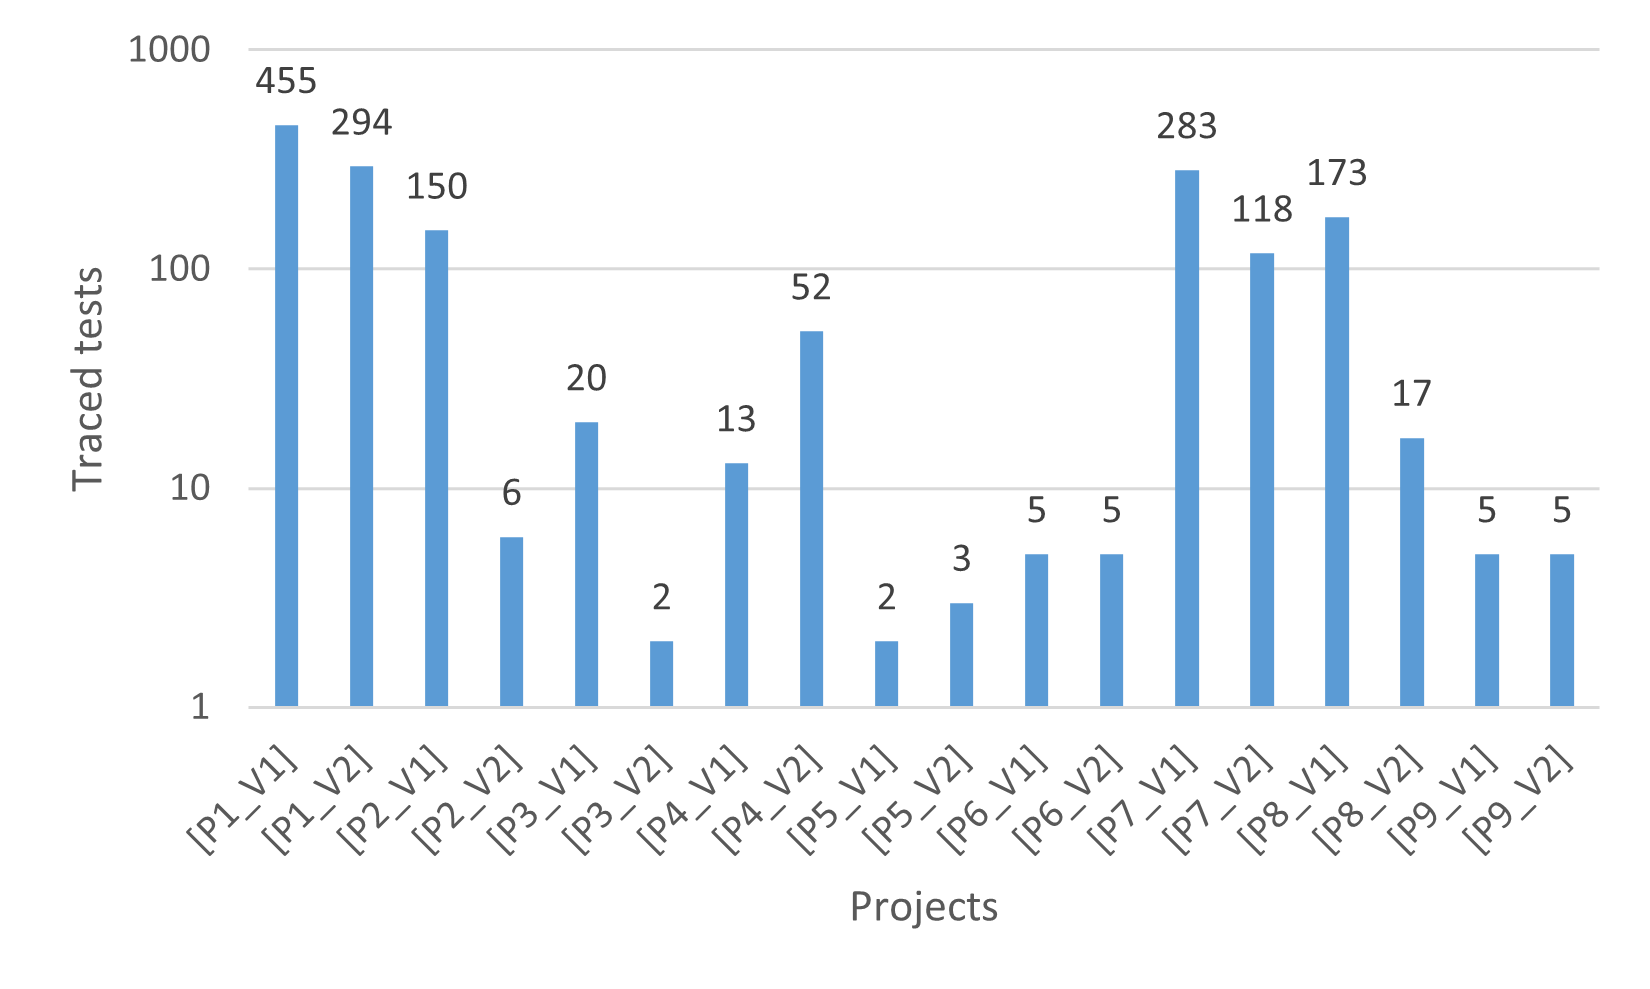
\includegraphics[width=0.7\textwidth]{img/tracedTests1.png}
%\vspace{-1em}
\caption{\red{Traced tests due to metamodel evolution in each project.}}
\label{fig:tracedTests}
%\vspace{-5mm}
\end{figure}

\begin{tcolorbox}[boxsep=-2pt]
\textbf{$\boldsymbol{RQ_1}$ insights:}
We could successfully trace the tests that must be executed before and after the co-evolution regardless of whether they are manually or automatically written. This would help developers to immediately check the code co-evolution by executing the subset of relevant traced tests among the whole test suite. 
\end{tcolorbox}

\subsubsection{RQ2}

After tracing the tests, we could execute them to observe their effect before and after co-evolution of the code. Table \ref{table:tracedTests} depicts the results for the original and evolved projects' versions. The second line gives the number of traced class tests and the rest of the lines categorizes the tests. \red{We overall observe no significant difference between projects with automatically generated tests and projects with manually tests.} 

The most interesting project is the first $[P1_{V1}]$ to $[P1_{V2}]$. Even though the tests decreased by \red{161 (455 - 294 from Figure \ref{fig:tracedTests}}), the number of passing tests decreased only by 9 (\red{106 - 97 from Table \ref{table:tracedTests}}). Regarding the error tests, they decreased by 155. However, the failing tests increased by 3 from 2 to 5\red{, as shown in Table \ref{table:tracedTests}. There was also the appearance of one failing test in $[P8]$.} These cases of increased failing tests indicate that the code co-evolution may be not completely behaviorally correct. 

Moreover, in the other projects $[P2][P3][P7][P8]$, many tests that existed in the original version were not in the evolved version due to the delete changes of the metamodels. This is actually a sign of behavioral correct co-evolution, as indeed the tests should be removed following the removal of the generated code for those deleted metamodel elements. 
\red{}In the rest of the projects $[P4][P5][P6][P9]$, roughly the same number of tests in the original version behaved the same in the evolved version, suggesting again a behaviorally correct co-evolution.
These results should help developers to further check the code co-evolution rather than simply accepting them in particular when it is fully automated. 

%\red{chech the three categrories of tests exists: 1/ in V1 and not in V2, 2/ in V1 and V2, 3/ in V2 and not V1.}

\begin{table*}[t]
%\begin{wraptable*}{r}{5.5cm}
\centering
\caption{Selected tests before and after code co-evolution.} %[Legend: Before (V1) -- After (V2) ]}
\label{table:tracedTests}
%
%\small
%\hspace*{-2em}
\resizebox{13cm}{!}{
\begin{tabular}{
@{\hskip3pt}c@{\hskip3pt}|c@{\hskip3pt}|c@{\hskip3pt}|c@{\hskip3pt}|c@{\hskip3pt}|c@{\hskip3pt}|c@{\hskip3pt}|c@{\hskip3pt}|| c@{\hskip3pt} |c@{\hskip3pt} }
\toprule 
Projects
& \begin{tabular}[c]{@{}l@{}}$[P1_{V1}]$ \\ to \\$[P1_{V2}]$\end{tabular}
& \begin{tabular}[c]{@{}l@{}}$[P2_{V1}]$ \\to \\$[P2_{V2}]$\end{tabular} &\begin{tabular}[c]{@{}l@{}} $[P3_{V1}]$ \\to\\ $[P3_{V2}]$ \end{tabular}
&\begin{tabular}[c]{@{}l@{}} $[P4_{V1}]$ \\to \\$[P4_{V2}]$\end{tabular}
&\begin{tabular}[c]{@{}l@{}} $[P5_{V1}]$\\ to\\ $[P5_{V2}]$\end{tabular}
& \begin{tabular}[c]{@{}l@{}}$[P6_{V1}]$ \\to\\ $[P6_{V2}]$\end{tabular} 
& \begin{tabular}[c]{@{}l@{}}$[P7_{V1}]$ \\to\\ $[P7_{V2}]$\end{tabular}
&\begin{tabular}[c]{@{}l@{}}$[P8_{V1}]$ \\to\\ $[P8_{V2}]$\end{tabular}
&\begin{tabular}[c]{@{}l@{}}$[P9_{V1}]$ \\to\\ $[P9_{V2}]$\end{tabular}\\ \midrule%{2-10}


\begin{tabular}[c]{@{}l@{}}$N^{o}$ class\\ tests \end{tabular} &  114 - 57 &  51 - 4   &   8 - 2  &  5 - 10   &   2 - 3   &   2 - 3   &   11 - 12  &   32 - 8  &   1 - 1    \\ \midrule \midrule


\begin{tabular}[c]{@{}l@{}}$N^{o}$ \\ pass\end{tabular} & \begin{tabular}[c]{@{}l@{}} 106 - 97 \end{tabular} & \begin{tabular}[c]{@{}l@{}}  124 - 0  \end{tabular} &\begin{tabular}[c]{@{}l@{}}  14 - 1  \end{tabular}  
&\begin{tabular}[c]{@{}l@{}}  10 - 22  \end{tabular}  
&\begin{tabular}[c]{@{}l@{}}  2 - 3 \end{tabular}  &
\begin{tabular}[c]{@{}l@{}}2 - 2\end{tabular} & \begin{tabular}[c]{@{}l@{}}206 - 68\end{tabular}
& \begin{tabular}[c]{@{}l@{}}146 - 10\end{tabular}
& \begin{tabular}[c]{@{}l@{}}5 - 5 \end{tabular}\\ \midrule


\begin{tabular}[c]{@{}l@{}}$N^{o}$\\ fail\end{tabular} & \begin{tabular}[c]{@{}l@{}} 2 - 5  \end{tabular} & \begin{tabular}[c]{@{}l@{}}  1 - 1  \end{tabular} &\begin{tabular}[c]{@{}l@{}}  0 - 0  \end{tabular}  
&\begin{tabular}[c]{@{}l@{}}  1 - 3  \end{tabular}  
&\begin{tabular}[c]{@{}l@{}}  0 - 0 \end{tabular}  
&\begin{tabular}[c]{@{}l@{}}0 - 0 \end{tabular}  & \begin{tabular}[c]{@{}l@{}}1 - 0\end{tabular}
&\begin{tabular}[c]{@{}l@{}}0 - 1 \end{tabular} 
&\begin{tabular}[c]{@{}l@{}}0 - 0\end{tabular} 
\\ \midrule


\begin{tabular}[c]{@{}l@{}}$N^{o}$\\ error\end{tabular} & \begin{tabular}[c]{@{}l@{}} 347 - 192 \end{tabular} & \begin{tabular}[c]{@{}l@{}}  25 - 5\end{tabular} &\begin{tabular}[c]{@{}l@{}}  6 - 1  \end{tabular}   
&\begin{tabular}[c]{@{}l@{}}  2 - 27  \end{tabular}  
&\begin{tabular}[c]{@{}l@{}}  0 - 0  \end{tabular}  &
\begin{tabular}[c]{@{}l@{}} 3 - 3  \end{tabular}  & \begin{tabular}[c]{@{}l@{}}76 - 50\end{tabular}
& \begin{tabular}[c]{@{}l@{}}27 - 6\end{tabular} 
& \begin{tabular}[c]{@{}l@{}}0 - 0\end{tabular} \\ 


\bottomrule
\end{tabular}
}
%\end{wraptable*} 
%\vspace{-1em}
\end{table*}

\begin{tcolorbox}[boxsep=-2pt]
\textbf{$\boldsymbol{RQ_2}$ insights:}
Our traced tests could hint in two projects that the co-evolution may not be entirely correct due to more failing tests and fewer passing tests. The rest of the project would hint on rather a correct co-evolution due to delete metamodel changes. Overall, automating the help for checking of the behavioral correctness of the code co-evolution for developers, regardless of whether they tests are manually or automatically written.  
\end{tcolorbox}



\subsubsection{RQ3}
With the traced tests due to the metamodel evolution, we can assess the gains in terms of test reduction and execution time compared to the whole test suite as a baseline. 
Indeed, rather than re-running the whole test suite both in the original and evolved versions, or worse, not considering the tests at all. We provide developers with a zoomed view of traced impacted tests by the metamodel evolution, hence, focusing on assessing the code co-evolution.  

The first line of Table \ref{table:tracedTests} already gives the number of traced impacted test classes that are always less than the original number of test classes. 

Table \ref{CaseStudies_CoEvolution_result} further illustrates the differences between the original test suite and the traced impacted tests in terms of number of test cases and execution time. Columns~2 and~3 give the number of original tests and of traced tests.
%
%Figure \ref{fig:testReduction} 
Column 4 depicts the gains in terms of test reduction percentage. On average, we observe a reduction gain of~88\% of test cases, varying from 46\% to 99.9\%. Out of 34612 tests in the 18 projects, we traced 1608 impacted tests representing an absolute 95\% reduction.

This naturally leads to a gain in terms of execution time reduction of the tests. 
Columns 5 and 6 give the execution times for the whole test cases and the traced ones. Herein, we measured the execution time through IDE runner for the Junit tests.
%Figure \ref{fig:testReduction}
Column 7 depicts the gains in execution time of the traced tests compared to the whole test suite. On average, we observe a reduction of 84\%, varying from 69\% to 99\%. 
%84.6\%
\red{Overall, we observe no significant difference in benefit of reducing tests and the gain in execution time between projects with automatically generated tests and projects with manually tests. Respectively, we observe a reduction gain in tests of 88\% versus~81\% and a reduction gain in execution of 82\% versus 95.5\%.} 


%\begin{table*}[t]
\begin{sidewaystable}
\centering
		\caption{Reduction gains of the number of traced tests and their execution time.}
		\label{CaseStudies_CoEvolution_result}
  %\hspace*{-4em}
	%\resizebox{15cm}{!} {
	\begin{tabular}{lcccccc}
		\toprule
  \begin{tabular}[c]{@{}l@{}}Projects co-evolved in response to the evolved \\ metamodels \end{tabular} 
  & \begin{tabular}[c]{@{}c@{}}$N^{o}$ of \\ tests\end{tabular}
  & \begin{tabular}[c]{@{}c@{}}$N^{o}$ of \\ traced tests\end{tabular}
  &  \begin{tabular}[c]{@{}c@{}}Reduction \\ gain \\ in tests \end{tabular}
  & \begin{tabular}[c]{@{}c@{}}Execution \\ time of \\ tests (s)\end{tabular} 
  &\begin{tabular}[c]{@{}c@{}}Execution \\ time of \\ traced tests (s)\end{tabular}
  &\begin{tabular}[c]{@{}c@{}}Reduction \\gain in \\ execution time \end{tabular} %& \begin{tabular}[c]{@{}c@{}}$N^{o}$ of total \\ direct errors \end{tabular}& \begin{tabular}[c]{@{}c@{}}$N^{o}$ of total \\ indirect errors \end{tabular}
  \\ \midrule		

$[P1_{V1}]$ ocl.examples.pivot & 7322 & 455
 &  \cellcolor{green!40}$\searrow$ 94\% &339.411  & 48.322 & \cellcolor{green!35}$\searrow$ 86\% \\ \midrule

$[P1_{V2}]$ ocl.examples.pivot & 4990 & 294 & \cellcolor{green!40}$\searrow$ 94\%  & 228.88  & 70.856 & \cellcolor{green!25}$\searrow$ 69\% \\ \midrule

$[P2_{V1}]$ ocl.examples.base & 2320 & 150 & \cellcolor{green!40}$\searrow$ 93.5\%  & 123.254 & 26.518& \cellcolor{green!30}$\searrow$ 79\% \\ \midrule

$[P2_{V2}]$ ocl.examples.base & 2133 & 6 & \cellcolor{green!40}$\searrow$ 99.7\%  & 99.105 & 5.294 & \cellcolor{green!40}$\searrow$ 95\% \\ \midrule


$[P3_{V1}]$ ocl.pivot & 8795 & 20 & \cellcolor{green!40}$\searrow$ 99.7\%  &859.69 &  0.497& \cellcolor{green!40}$\searrow$ 99\% \\ \midrule

$[P3_{V2}]$ ocl.pivot & 6396 & 2 & \cellcolor{green!40}$\searrow$ 99.9\%  & 261.792 & 12.133 & \cellcolor{green!40}$\searrow$ 95\% \\ \midrule

$[P4_{V1}]$ papyrus.infra.extendedtypes & 135 & 13 & \cellcolor{green!40}$\searrow$ 90\%  &16.94 &  2.924& \cellcolor{green!35}$\searrow$ 83\% \\ \midrule

$[P4_{V2}]$ papyrus.infra.extendedtypes & 248 & 52 & \cellcolor{green!30}$\searrow$ 79\%  & 17.076 & 2.957& \cellcolor{green!35}$\searrow$ 83\% \\\midrule

$[P5_{V1}]$ papyrus.infra.extendedtypes.emf & 104 & 2 & \cellcolor{green!40}$\searrow$ 98\%  & 6.912& 2.11& \cellcolor{green!25}$\searrow$ 70\% \\ \midrule
$[P5_{V2}]$ papyrus.infra.extendedtypes.emf & 104 & 3  & \cellcolor{green!40}$\searrow$ 97\%  & 7.31& 1.802 & \cellcolor{green!25}$\searrow$ 75\% \\ \midrule

$[P6_{V1}]$ papyrus.uml.tools.extendedtypes & 75 & 5 & \cellcolor{green!40}$\searrow$ 93\%  &5.9 & 1.505 & \cellcolor{green!25}$\searrow$ 75\% \\ \midrule

$[P6_{V2}]$ papyrus.uml.tools.extendedtypes & 75 & 5 &  \cellcolor{green!40}$\searrow$ 93\% & 6.246 & 1.099& \cellcolor{green!35}$\searrow$ 82\% \\ \midrule

$[P7_{V1}]$ org.eclipse.modisco.infra.discovery.benchmark& 524 & 283 & \cellcolor{green!10}$\searrow$ 46\%  & 7.332 & 2.04 & \cellcolor{green!25}$\searrow$ 73\%  \\ \midrule

$[P7_{V2}]$ org.eclipse.modisco.infra.discovery.benchmark& 619 & 118 & \cellcolor{green!35}$\searrow$ 81\%  & 14.534 &4.107  & \cellcolor{green!25}$\searrow$ 72\% \\% \midrule
\midrule

$[P8_{V1}]$ org.eclipse.emf.test.core& 322 & 173 & \cellcolor{green!10}$\searrow$ 46\%  & 176.372 & 2.908 & \cellcolor{green!40}$\searrow$ 98\%  \\ 
\midrule

$[P8_{V2}]$ org.eclipse.emf.test.core& 322 & 17 & \cellcolor{green!40}$\searrow$ 94\%  & 157.041& 0.346 & \cellcolor{green!40}$\searrow$ 99\%  \\ 

\midrule

$[P9_{V1}]$ org.eclipse.emf.test.xml& 64 & 5 & \cellcolor{green!40}$\searrow$ 92\%  & 3.764 & 0.247 & \cellcolor{green!40}$\searrow$ 93\%  \\ 
\midrule

$[P9_{V2}]$ org.eclipse.emf.test.xml& 64 & 5 & \cellcolor{green!40}$\searrow$ 92\%  & 3.193 & 0.257 & \cellcolor{green!40}$\searrow$ 92\%  \\ 



   \bottomrule		
\end{tabular}
%}

%\end{table*}
\end{sidewaystable}
\begin{comment}

\begin{figure}[t]
\centering
%\hspace*{-2em}
\includegraphics[width=0.5\textwidth]{img/.png}
%\vspace{-1em}
\caption{Reduction gains of traced tests from the whole test suite in each project.}
\label{fig:gain1}
%\vspace{-5mm}
\end{figure}

\begin{figure}[t]
\centering
%\hspace*{-2em}
\includegraphics[width=0.5\textwidth]{img/.png}
%\vspace{-1em}
\caption{Execution gains of traced tests from the whole test suite in each project.}
\label{fig:gain2}
%\vspace{-5mm}
\end{figure}
\end{comment}


\begin{tcolorbox}[boxsep=-2pt]
\textbf{$\boldsymbol{RQ_3}$ insights:}
Tracing the metamodel evolution changes up to the impacted tests allows assessing the co-evolution behavioral correctness, while %Doing so, our approach gains represent
gaining, on average, a reduction of 88\% in the number of tests and 84\% in execution time. The reduction gains are similar with no significant difference regardless of whether the tests are manually or automatically written.
\end{tcolorbox}




\section{Threats to Validity}\label{threat}
\noindent This section discusses threats to validity \cite{wohlin2012experimentation}.

\subsection{Internal Validity.}
To be able to trace the impact of metamodel changes to the tests, we had to have a test suite in the selected projects. However, we observed that the Eclipse projects relying on metamodels do not come with the test suite. This was not only the case of OCL\cite{MDTOCL}, papyrus \cite{MDTPapyrus} or Modisco \cite{MDTModisco}, but also other Eclipse languages \cite{UML241,BPMN2}. Therefore, we were obliged to generate the test suite with a state-of-the-art available tool EvoSuite \cite{fraser2011evosuite}. 
Even though, automatic test generation is a best practice, there is the risk of having tests that are different from manually written tests. 
However, this does not pose a risk to our approach as the main algorithm of our approach is generic and would be able to trace the impact of a metamodel change in the same way for both automatically generated tests as well as manually written tests. \red{This is what we observed with the fourth EMF case study having manually written tests. Indeed, the overall results of tracing tests and reduction gains were not significantly different in all case studies regardless of whether the tests are automatically generated or manually written.} 
The main risk is related to the behavioral correctness of the code co-evolution. To check it, we require unit tests that target single methods. 
However, automatic test generation can even be more advantageous herein. Indeed, it generates tests for all public methods, whereas developers tend to manually write only few tests for some targeted methods. Thus, if relying only on manually written tests, there is a high risk of not assessing the behavioral correctness of many cases of code co-evolutions that are not covered by test cases. 
This is mitigated by relying on EvoSuite that generates a full test suite of unit tests with Junit assertions. This tool has shown his efficiency in test generation as a state-of-the-art tool~\cite{DANGLOT2019110398,https://doi.org/10.1002/stvr.1601}. \red{Indeed, this is observed when computing the coverage metric for each of our considered projects (see Table \ref{table:coverage}). The highest coverage is on projects with automatically generated tests and the lowest coverage is on the two projects with manually written tests.}
 
Therefore, our approach not only checks the correctness of the code co-evolution with the traced tests, but also favors the best practice of tests generation in each release of a software language after its metamodel evolution.
%\red{Furthermore, as we studied releases, there is a risk that a test verdict is not only impacted by a code co-evolution but also by other code changes. This, is why we provide a diagnostic for developers with the traced tests as starting point to investigate. Nonetheless, if our approach is performed in a continuous integration mode after each code co-evolution, the traced tests verdicts will solely be due to the given metamodel change.} 

Finally, as our tracing approach relies on the quality of detected metamodel changes, we analyzed, in our evaluation, each detected change and checked whether it occurred between the original and evolved metamodels. This alleviates the risk of relying on an incorrect metamodel change that would degrade the tracing of the impacted tests by metamodel changes, i.e., not tracing an impacted test by a non-considered metamodel change. 
%we plan to run an experiment with devolopers
\red{In addition, as we did not have the ground truth, we could not report on the precision and recall of our approach. 
However, our approach uses the Code Call Graph and starts from the generated code elements corresponding to the evolved metamodel elements to recursively trace back any existing tests. Thus, by design we actually detect all the impacted tests that must be traced. To test that our algorithm does not miss any impacted test, and does not trace non-impacted tests, we manually verified the ground truth for our smallest data set projects $[P6]$ and $[P9]$, because they have fewer tests and are less complex. We checked for every metamodel change all the impacted tests and we found that our approach traces all of them. 
Further evaluation on a ground truth is left for future work.} 

\subsection{External Validity.} 
We implemented and evaluated our approach for EMF/Ecore metamodels and Java code with Junit tests. Other languages, such as C\# or C++, use a different syntax, but conceptually use the same constructions as in Java.
Although we think that the tracing would be applicable for other languages, we cannot generalize our results. Further experimentation on other languages is necessary. However, the only requirement to apply our approach to other languages is to have access to the ASTs of the parsed code and tests, and to adapt our tracing of the tests in the build call graph. 
%
Moreover, our evaluation was performed on Eclipse projects from five languages. Thus, we cannot generalize our findings to all software languages or DSLs. We also cannot generalize our results on manually written tests, in particular the test verdicts of the traced tests, i.e., pass, fail, and error. Further experimentation remains necessary and is left for future work. 

\subsection{Conclusion Validity.}
Our evaluation gave promising results, showing that we could trace the impact of metamodel changes till the tests, and hence, check the behavioral correctness of the code co-evolution in practice for real-world projects. 
However, even though we evaluated our approach on 18 projects of metamodel evolution and code co-evolution with automatically generated tests and manually written tests, further evaluation is needed on more case studies to have more insights and statistical evidence. \red{Finally, our user study experiment suggesting our approach usefulness needs to be replicated with more participants.} 
